\chapter{Metode}
\textit{I dette kapitel beskrives metoden for at besvare problemformuleringen, herunder udviklingen af et regelbaseret system til risikovurdering og evaluering af systemets anvendelighed.}

\section{Formål}
Formålet er at undersøge, hvilken anvendelighed et regelbaseret system har til risikovurdering af lægemiddelskift, med henblik på at gøre den nuværende proces mindre personafhængig og sårbar. Systemet skal på baggrund af risikofaktorer, der anvendes i den nuværende vurdering, foretaget af ATC-ansvarlige medarbejder, og problemstillinger relateret til lægemiddelskift, vurderer risikoen ved lægemiddelskift. Ved vurdering af risiko er det muligt for ATC-ansvarlige medarbejdere at vurdere i hvilke tilfælde de skal være særligt opmærksomme på lægemiddelskiftet. Denne viden kan anvendes til udarbejdelse af Lægemiddel Nyt, hvis formål er, at informere den enkelte hospitalsafdeling om, hvornår de skal være særligt opmærksomme på et lægemiddelskift, da dette kan være kompleks at implementere.

%\section{Metodebeskrivelse}
%For at udvikle et system til risikovurdering af lægemiddelskift skal den nødvendige data indsamles 


%Udviklingen af et system til risikovurdering af lægemiddelskift gennemgår forskellige udviklingstrin, herunder indsamling af data, udvælgelse af risikofaktorer og vægtning af disse, præprocessering af data, design, implementering og test samt evaluering af systemet. Udviklingsprocessen har foregået som en iterativproces, hvor der har været overlap mellem de enkelte trin. Udviklingstrinene fremgår af Figur \ref{fig:metode}. 

%\begin{figure}[H]\centering	\includegraphics[width=1\textwidth]{billeder/udviklingstrin.png} 
	%\caption{Udviklingstrin for processen.}
	%\label{fig:metode}  
%\end{figure}
%\vspace{-0.5cm}

%Af Figur \ref{fig:metode} illustreres de forskellige udviklingstrin som gennemgås ved udviklingen af et system til risikovurdering af lægemiddelskift. Indsamling af data danner grundlaget for den næste proces i forhold til udvælgelse af risikofaktorer. Risikofaktorer er udvalgt på baggrund af indsamlet data og litteratur. Disse vægtes efterfølgende af en ekspert inden for området. Dernæst foretages præprocessering af data for at gøre data homogent og sammenligneligt. Efterfølgende designes systemet som omhandler design af risikovurdering. Herefter implementeres designet af systemet. Systemet er efterfølge unit-testet. Til sidst evalueres systemets anvendelighed.

\section{Dataindsamling}
Data vedrørende lægemiddelskift for SRN er udtrukket fra sygehusapoteksportalen og sorteret af en medarbejder på SRN i forhold til relevans for udarbejdelsen af skiftelister, beskrivelsen af dette fremgår af Appendiks \ref{App:Skiftelister}. Skiftelisterne er gældende for skift i år 2014 (n=231), 2015 (n=160), 2016 (n=318), 2017 (n=229) og 2018 (n=244). Hver skifteliste indeholder oplysninger om lægemidlets ATC-kode, navn, dispenseringsform og styrke for forgående år og året for skiftet, hvilket fremgår af Figur \ref{fig:Input}.

\begin{figure}[H]\centering
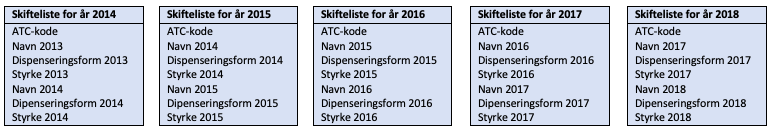
\includegraphics[width=1\textwidth]{billeder/Input1.png} 
	\caption{Skiftelister for år 2014, 2015, 2016, 2017 og 2018, indeholdende oplysninger om ATC-kode, lægemidlets navn, dispenseringsform og styrke.}
	\label{fig:Input}  
\end{figure}

Skiftelisterne kombineres med udbudsmateriale, som fremgår af \ref{fig:Input2}, for lægemiddelskift, der er udtrukket fra sygehusapoteksportalen, og indeholder oplysninger om blandt andet ATC-kode, lægemidlets navn, styrke og dispenseringsform samt priser og hvorvidt lægemidlet indgår i Medicinrådets behandlingsvejledning for de udbud som er gældende for for det kommende år. Hvis lægemidlet indgår i Medicinrådets behandlingsvejledning er det lovmæssigt bestemt at disse skal anvendes som standardbehandling~\citep{Medicinradet2018}. Ligeledes kombineres skiftelisterne med viden omkring kritiske ATC-koder, der er indsamlet af SRN i forbindelse med problemstillinger vedrørende lægemiddelskift, som omfatter ATC-koderne, som fremgår af Figur \ref{fig:Input2}, og risikolægemidler som er indsamlet af Amgros, som indeholder ATC-kode og lægemidlets navn. Risikolægemidler er lægemidler som f.eks. kræver et ekstra personalemæssigt ressourcetræk i forbindelse med lægemiddelskift samt lægemidler, hvor der er øget risiko for utilsigtede hændelser~\citep{Amgros}. 

\begin{figure}[H]\centering
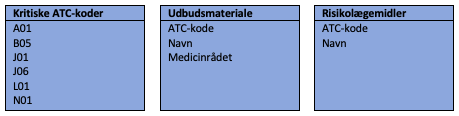
\includegraphics[width=0.6\textwidth]{billeder/Input2.png} 
	\caption{Kritiske ATC-koder, udbudsmateriale og risikolægemidler, der kombineres med skiftelister på baggrund af ATC-kode eller lægemidlets navn.}
	\label{fig:Input2}  
\end{figure}

\section{Risikofaktorer og vægtning}
Risikofaktorer er udvalgt ud fra den nuværende vurdering af ATC-ansvarlige medarbejdere, som er beskrevet af Afsnit \ref{sec:ImpLaeg}. Litteratur som beskriver risikofaktorer som har ledt til medicineringsfejl i klinikken som følge af lægemiddelskift, hvilket er beskrevet af Afsnit \ref{sec:ProblemLaeg}. Dokumenterede ATC-koder af SRN, som har ledt til problemstillinger vedrørende lægemiddelskift og derfor anses som kritiske~\citep{SRN}. Risikolægemidler, der overvåges særligt af Amgros, som er kritiske, hvis de ender i restordre på grund af f.eks. leveringesvigt \citep{Amgros}. Risikofaktorerne er efterfølgende vægtet af en ekspert inden for området, hvoraf en vægtning på 1 anses som værende af mindre betydning for implementering af lægemiddelskift og 5 anses som værende af stor betydning. Risikofaktorer og deres vægt samt begrundelse for valg fremgår af Tabel \ref{table:features}.

\begin{longtable}{p{3.5cm}| p{1.0cm} | p{9.2cm}}
	\caption{Risikofaktorer} \vspace{0.2cm}
	\label{table:features} \\
\cellcolor[HTML]{C0C0C0} {\textbf{Risikofaktor}} & \cellcolor[HTML]{C0C0C0} {\textbf{Vægt}} & \cellcolor[HTML]{C0C0C0} {\textbf{Begrundelse}} \\ \hline
\textbf{Navn} & 1 & Den hyppigste årsag til medicineringsfejl ved generisk substitution er ordinering af det forkerte lægemiddel, hvilket typisk skyldes at lægemidlets navn lignede og/eller havde et svært navn~\citep{Hakonsen2010}. \\  \hline 
\textbf{Look-a-like} & 2 & Look-a-like har påvist at kunne prædisponeres til medicineringsfejl~\citep{Wittich2014}. Dette kan have patientsikkerhedsmæssige konsekvenser, hvis f.eks. smertestillende panodil forveksles med plendil til behandling af forhøjet blodtryk ~\citep{DanskSelskabforPatientsikkerhed2009}.\\  \hline 
\textbf{Dispenseringsform} & 2 & Dispenseringsform giver anledning til medicineringsfejl i forbindelse med ordination~\citep{Agrawal2009}. Ved ordination af det forkerte lægemiddel, grundet navneforveksling, kan dette give anledning til fejl i dispenseringsform~\citep{DanskSelskabforPatientsikkerhed2009}, hvilket har betydning for virkningen af lægemidlet.
\\ \hline 
\textbf{Styrke} & 2 & Styrke kan medføre medicineringsfejl ved ordination ved f.eks. forkert styrkeberegning~\citep{Agrawal2009}, hvorfor det er vigtigt at være opmærksom på  ændring i styrke for at undgå beregningsfejl, hvormed patienten kan risikere at få en højere eller lavere styrke end ordineret.\\ \hline
\textbf{Risikolægemidler} & 3 & Disse overvåges særligt af Amgros, da de er kritiske hvis de ender i restordre, hvorfor det anbefales at have et lager af disse lægemidler i op til 8 uger~\citep{Amgros}. Yderligere kræver nogle af lægemidlerne et ekstra personalemæssigt ressourcetræk i forbindelse med skift og er i øget risiko for utilsigtede hændelser~\citep{Amgros}. \\ \hline 
\textbf{ATC-grupper} & 5 & ATC-grupper såsom, A10, B05, J01, J06, L01 og N01 har givet anledning til problemstillinger vedrørende lægemiddelskift og er derfor defineret af SRN som kritiske \citep{SRN}. \\ \hline 
\textbf{Medicinråd} & 5 & Lægemidler som indgår i medicinrådets behandlingsvejledninger er lægemidler som er besluttet at anvendes som standardbehandling~\citep{Medicinradet2018}. Disse vurderes i forhold til effekt, eksisterende behandling og pris~\citep{Medicinradet2018}. For lægemidler som indgår i Medicinrådet er der ofte mange penge og spare, hvorfor disse skal implementeres hurtigt. \\ \hline 
    \end{longtable}

\section{Præprocessering}
Præprocessering af data er nødvendigt, da data er tekstbaseret og indskrevet manuelt og derfor ikke sammenligneligt. Det er forskelligt om data er skrevet med majuskel eller minuskel, hvorfor det er valgt at ændre alt data til minuskel. Ligeledes er forkortelser udskrevet og tegnsætning fjernet for at gøre data generaliserbart. Det varierer for styrke om der anvendes mellemrum mellem tal og enheder, hvorfor mellemrum er fjernet.

Det er antaget for tomme tekstfelter at intet er ændret, hvormed data fra enten tidligere år eller for det kommende skift er gældende. For lægemidlets navn er det antaget at dette er ens, hvis præfiks er uændret, hvorfor suffiks er fjernet. Lægemidler med ens præfiks, men forskellig suffiks, kan give anledning til forskellige dispenseringsformer eller styrker. Hvis dette er tilfældet vil dette opdages i forbindelse med sammenligning af dispenseringsform og styrke. Synonymer, såsom f.eks. filmovertrukne eller overtrukne, er fjernet og angivet som tabellet. 

\section{Design}
%\textcolor{red}{Tilføj: Hvilke overvejelser har jeg gjort i design i forhold til at gøre systemet generealiserbart?} \\
Risikovurderingen er designet som if-then-else statements som danner grundlag for risikovurderingen. For hvert statement vurderes én eller flere risikofaktorer i forhold til om et statement er sandt eller falsk. Ud fra antallet af sande statements beregnes risikoscoren ud fra Ligning \ref{equ:risikoscore} på baggrund af den totale vægt af alle matchende risikofaktorer og den totale vægt af alle risikofaktorer.

\begin{equation}  \label{equ:risikoscore}
Riskoscore = \frac{\mbox{\textit{Totale vægt af alle matchende risikofaktorer}}}{\mbox{\textit{Totale vægt af alle risikofaktorer}}} * 100
\end{equation}

Risikoscoren er angivet som en procentdel, hvorved der er en bedre beslutningsgrundlag for at vurdere risikoscoren. En høj risikoscore vil betyde at de risikofaktorer, som gør sig gældende har stor betydning for lægemiddelskiftet. Hvis risikoscoren modsat er lille vil denne have en mindre betydning for lægemiddelskiftet. Det skal på denne måde være muligt for de ATC-ansvarlige medarbejdere på SRN at skelne, hvilke tilfælde de skal være ekstra opmærksomme på lægemiddelskift i forhold til at der kræves yderligere information til klinikken ved udarbejdelsen af Lægemiddel Nyt.  

Til design af look-a-like lægemidler, der sammenligner hvorvidt et lægemiddels navn for det kommende skifteår ligner et andet lægemiddel, som er registreret ved tidligere lægemiddelskift, beregnes Levenshtein distance. Levenshtein distance er et udtryk for det minimale antal af operationer, herunder slette, indføre eller erstatte, der kræves for at ændre et ord til et andet. Denne distance beregnes ud fra Ligning \ref{equ:LevDistance} på baggrund af det minimale antal af tilføjede, slettede og erstattede bogstaver der kræves for at ændre et ord til et andet samt den maksimale længde af de to ord som sammenlignes. 

\begin{equation} \label{equ:LevDistance}
\mbox{\textit{Distance}} = 1 - \frac{\mbox{\textit{min(antal af tilføjede, slettede og erstattede bogstaver)}}}{\mbox{\textit{max(længde af ord der sammenlignes)}}}   
\end{equation}

Outputtet er designet ud fra, hvordan den nuværende vurdering af lægemiddelskift foregår. Da skiftelisterne er udarbejdet i excel-filer og de ATC-ansvarlige medarbejdere er velkendt med denne proces er det valgt at outputtet visualiseres i allerede eksisterende excel-filer. Udover de nuværende data tilføjes en ekstra kolonne til excel-filen, som indeholder risikoscore og begrundelse for denne score. Designet af outputtet fremgår af Figur \ref{fig:Output}.

\begin{figure}[H]\centering
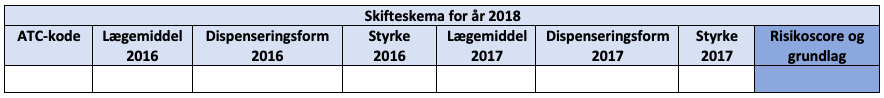
\includegraphics[width=1\textwidth]{billeder/Output.png} 
	\caption{Design af output. De lyseblå kasser symboliserer allerede eksisterende kolonner, hvor den mørkeblå kasse er tilføjet og indeholder output.}
	\label{fig:Output}  
\end{figure}

\newpage
\section{Implementering og test}
*** Levenshtein distance  ***
Systemet er implementeret i NetBeans, som er et Integrated Development Environment (IDE) til java.  Java Excel API (JExcelApi) og Apache POI er tilføjet til biblioteket for at kunne indlæse Microsoft dokumenter. For at kunne håndtere æ, ø og å er tegnsættet ændret i NetBeans IDE til ISO-8859-15. 

\section{Evaluering}
Systemet blevet evalueret af ATC-ansvarlige medarbejder af i forhold til at teste selve systemets anvendelighed samt hvor anvendeligt systemet er for de ATC-ansvarlige medarbejdere. En introduktion til systemet, hvilket fremgår af Appendiks \ref{App}, blev givet inden det blev evalueret for at sikre at systemets formål var forstået.

Systemets anvendelighed blev testet ved at vurdere 33 lægemiddelskift udvalgt fra skift i år 2016, 2017 og 2018, hvilket fremgår af Appendiks~\ref{App:Evaluering}. Udvælgelsen er vurderet af en ekspert på området og udvalgt i forhold til at repræsentere forskellige risikoscores og begrundelser for disse.
De enkelte lægemiddelskift er vurderet i forhold til, hvornår der kræves uddybende information til klinikken via Lægemiddel Nyt.
Efterfølgende blev sammenhængen mellem vurderingen af lægemiddelskiftene og hvilke lægemidler, der var uddybende information i Lægemiddel Nyt fra år 2016, 2017 og 2018 test i en XXX.

Dernæst blev anvendeligheden af systemet vurderes i forhold til 

%Systemets anvendelighed er evalueret af 12 ATC-ansvarlige medarbejdere, som står for vurderingen af lægemiddelskift. For at give de ATC-ansvarlige medarbejdere et grundlag for at evaluere systemet afprøves systemet.

%Systemet afprøves ved at vurdere 30 repræsentative lægemiddelskift for skift i år 2016, 2017 og 2018, som fremgår af Appendiks~\ref{App:Evaluering}, på en skala fra 0 til 5, i forhold til, hvornår de ATC-ansvarlige medarbejdere vurderer at der skal være særlig opmærksomhed rettet mod lægemiddelskiftet. Vurderes et lægemiddelskift til 0 vil dette betyde at lægemiddelskiftet kræver mindre opmærksomhed, hvorimod 5 kræver større opmærksomhed ved implementering. Denne vurderingen sammenlignes med Lægemiddel Nyt fra år 2016, 2017 og 2018 i forhold til at se om de lægemiddelskift,som vurderes til at kræve større opmærksomhed, er beskrevet yderligere i Lægemiddel Nyt. Vurderingen af lægemiddelskift foregår individuelt og tager udgangspunkt i outputtet fra systemet, såsom risikoscore, ændringer i lægemidlets navn, dispenseringsform, styrke, look-a-like, kritisk ATC-kode, risikolægemiddel og Medicinrådet. 

%Efter de ATC-ansvarlige har fået kendskab til systemet gives der feedback på systemets anvendelighed. Dette gøres i grupper af to, hvor der tages stillingen til systemets anvendelighed og videreudvikling af systemet. Efterfølgende vil anvendeligheden og videreudvikling diskuteres af samlet. 




